\documentclass[tikz, border=6pt]{standalone}
\usepackage[T1]{fontenc}
\usepackage{lmodern}
\usepackage{amsmath,amssymb,bm}
\usepackage{lmodern}
\usetikzlibrary{arrows.meta}
\definecolor{Blue}{HTML}{3A76D8}
\definecolor{Green}{HTML}{3BA55C}
\definecolor{Orange}{HTML}{EE8133}
\definecolor{Red}{HTML}{DF4B4B}
\definecolor{Ink}{HTML}{1F2937}
\tikzset{
  dot/.style={circle, fill, inner sep=0pt, minimum size=4.5pt},
}
\begin{document}
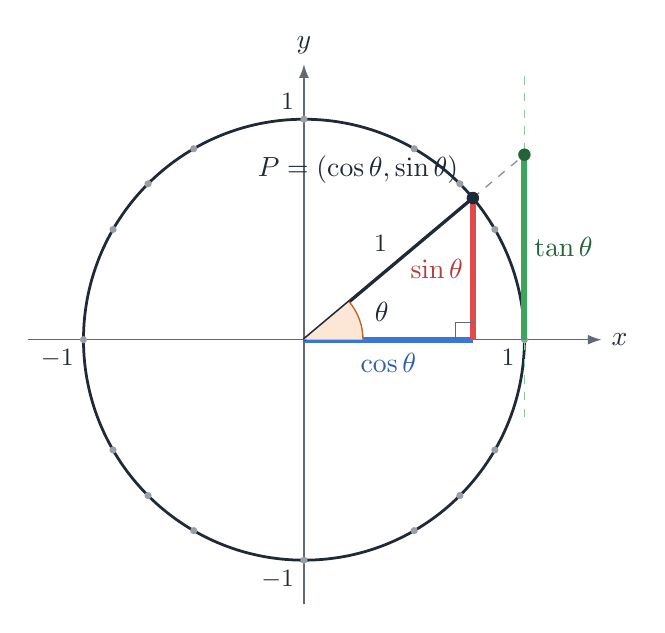
\begin{tikzpicture}[color=Ink, line width=0.5pt, >={Latex[length=5pt, width=3.6pt]}, line join=round]
  \draw[->, color=Ink!70] (-3.5,0) -- (3.78,0);
  \draw[->, color=Ink!70] (0,-3.36) -- (0,3.5);
  \node[anchor=west] at (3.78,0) {$x$};
  \node[anchor=south] at (0,3.5) {$y$};
  \draw[line width=1pt] (0,0) circle[radius=2.8cm];
  \node[dot, fill=Ink!45, minimum size=2.6pt] at (2.8,0) {};
  \node[dot, fill=Ink!45, minimum size=2.6pt] at (2.4249,1.4) {};
  \node[dot, fill=Ink!45, minimum size=2.6pt] at (1.4,2.4249) {};
  \node[dot, fill=Ink!45, minimum size=2.6pt] at (0,2.8) {};
  \node[dot, fill=Ink!45, minimum size=2.6pt] at (-1.4,2.4249) {};
  \node[dot, fill=Ink!45, minimum size=2.6pt] at (-2.4249,1.4) {};
  \node[dot, fill=Ink!45, minimum size=2.6pt] at (-2.8,0) {};
  \node[dot, fill=Ink!45, minimum size=2.6pt] at (-2.4249,-1.4) {};
  \node[dot, fill=Ink!45, minimum size=2.6pt] at (-1.4,-2.4249) {};
  \node[dot, fill=Ink!45, minimum size=2.6pt] at (0,-2.8) {};
  \node[dot, fill=Ink!45, minimum size=2.6pt] at (1.4,-2.4249) {};
  \node[dot, fill=Ink!45, minimum size=2.6pt] at (2.4249,-1.4) {};
  \node[dot, fill=Ink!45, minimum size=2.6pt] at (1.9799,1.9799) {};
  \node[dot, fill=Ink!45, minimum size=2.6pt] at (-1.9799,1.9799) {};
  \node[dot, fill=Ink!45, minimum size=2.6pt] at (-1.9799,-1.9799) {};
  \node[dot, fill=Ink!45, minimum size=2.6pt] at (1.9799,-1.9799) {};
  \node[anchor=north east, font=\small] at (2.8,0) {$1$};
  \node[anchor=north east, font=\small] at (-2.8,0) {$-1$};
  \node[anchor=south east, font=\small] at (0,2.8) {$1$};
  \node[anchor=north east, font=\small] at (0,-2.8) {$-1$};
  \draw[color=Green!60, dashed] (2.8,-0.98) -- (2.8,3.36);
  \draw[color=Ink!50, dashed] (2.1449,1.7998) -- (2.8,2.3495);
  \draw[color=Blue, line width=2.2pt] (0,0) -- (2.1449,0);
  \draw[color=Red, line width=2.2pt] (2.1449,0) -- (2.1449,1.7998);
  \draw[color=Green, line width=2.2pt] (2.8,0) -- (2.8,2.3495);
  \node[anchor=north, text=Blue!80!black, yshift=-0.05cm] at (1.0725,0) {$\cos\theta$};
  \node[anchor=east, text=Red!80!black] at (2.1449,0.8999) {$\sin\theta$};
  \node[anchor=west, text=Green!60!black] at (2.8,1.1747) {$\tan\theta$};
  \draw[line width=1.2pt] (0,0) -- (2.1449,1.7998);
  \node[anchor=south east, font=\small] at (1.1797,0.9899) {$1$};
  \fill[color=Orange!20] (0,0) -- (0.75,0) arc[start angle=0, end angle=40, radius=0.75cm] -- cycle;
  \draw[color=Orange!80!black] (0.75,0) arc[start angle=0, end angle=40, radius=0.75cm];
  \node at (0.9867,0.3591) {$\theta$};
  \draw[color=Ink!70] (1.9249,0) -- (1.9249,0.22) -- (2.1449,0.22);
  \node[dot, fill=Ink, label={above left:{$P = (\cos\theta, \sin\theta)$}}] at (2.1449,1.7998) {};
  \node[dot, fill=Green!60!black] at (2.8,2.3495) {};
\end{tikzpicture}
\end{document}
